\documentclass[12pt]{beamer}
\usetheme{CambridgeUS}
\usepackage[utf8]{inputenc}
\usepackage[spanish]{babel}
\usepackage{amsmath}
\usepackage{amsfonts}
\usepackage{amssymb}
\usepackage{graphicx}
\usepackage{ragged2e}
\setbeamertemplate{navigation symbols}{} 
\author[Kevin García - Alejandro Vargas]{Kevin García 1533173 \newline Alejandro Vargas 1525953}
\title[Tarea 5: Regresión Robusta]{Tarea 5:Diagnósticos en el Análisis de Regresión, Regresión a Través del Origen y Regresión Robusta}



%\setbeamercovered{transparent} 
%\setbeamertemplate{navigation symbols}{} 
%\logo{} 
%\institute{} 
%\date{} 
%\subject{} 
\begin{document}
\justify
\begin{frame}
\titlepage
\end{frame}

%\begin{frame}
%\tableofcontents
%\end{frame}
\begin{frame}
\frametitle{Introducción}
~\\En esta presentación se tratara de encontrar un modelo lineal adecuado, para predecir la cantidad de $PM_{2.5}$ a partir de la cantidad de $PM_{10}$, para ello se ajustara un modelo simple por MCO y se llevaran a cabo pruebas de diagnostico para detectar e identificar puntos con altos residuales, atípicos, influyentes o de alto leverage, y se tratará de mejorar el modelo llevando a cabo un modelo ajustado que pase por el origen, al cuál se le aplicaran nuevamente las pruebas de diagnostico y se le evaluaran el cumplimiento de los supuestos.Finalmente, se aplicara regresión robusta y se compararan todos los modelos, eligiendo el mejor o el más adecuado.
\end{frame}

\begin{frame}
\frametitle{Definiciones}
~\\El material particulado respirable presente en la atmósfera de nuestras ciudades en forma sólida o líquida (polvo, cenizas, hollín, partículas metálicas, cemento y polen, entre otras) se puede dividir, según su tamaño, en dos grupos principales. A las de diámetro aerodinámico igual o inferior a los 10 $\mu m$ o 10 micrómetros (1 $\mu m$ corresponde a la milésima parte de un milímetro) se las denomina $PM_{10}$ (partículas respirables) y a la fracción respirable más pequeña, $PM_{2.5}$ (partículas finas). Estas últimas están constituidas por aquellas partículas de diámetro aerodinámico inferior o igual a los 2.5 micrómetros, es decir, son 100 veces más delgadas que un cabello humano, además son más peligrosas, ya que, al ser inhaladas, pueden alcanzar las zonas periféricas de los bronquiolos y alterar el intercambio pulmonar de gases.
\end{frame}

\begin{frame}
\frametitle{Modelo Ajustado}
~\\~\\Para ajustar un modelo lineal para estas partículas, decidimos que la variable independiente o regresora fuera el $PM_{10}$ y la variable dependiente fuera el $PM_{2.5}$, se hizo esta selección, ya que las partículas con un diámetro menor o igual a 10 micrómetros son más fáciles de medir que las de diámetro menor o igual a 2.5 micrómetros, y la idea es que se ahorren costos y esfuerzo humano adicional, midiendo solo las partículas $PM_{10}$ (que son un poco más grandes) y a partir de ellas logren obtener una buena estimación para las partículas $PM_{2.5}$.
\end{frame}

\begin{frame}
\frametitle{Modelo Ajustado}
~\\Teniendo en cuenta lo anterior, el modelo planteado es:
$$PM_{2.5}=\beta_{0}+\beta_{1}PM_{10}$$
~\\El modelo ajustado, usando MCO es:
$$\hat{PM_{2.5}}=-4.29990+0.45776PM_{10}$$
\end{frame}

\begin{frame}
\frametitle{Bondad del modelo}
~\\Para este modelo ajustado, tenemos los siguientes resultados que nos ayudaran a juzgar que tan bueno es:
\begin{center}
~\\\begin{tabular}{|c|c|c|c|c|}
\hline 
 & Estimación & Desviación Estandár & Estadistico T & P valor \\ 
\hline 
$\beta_{0}$ & -4.29990 & 1.27362 & -3.376 & 0.000916 \\ 
\hline 
$\beta_{1}$ & 0.45776 & 0.03051 & 15.001 & $<2e-16$ \\ 
\hline 
\end{tabular} 
\end{center}
~\\En la tabla anterior se puede apreciar que ambas estimaciones de los coeficientes son significativas a muy bajos niveles de $\alpha$,ya que el p valor para ambos es casi cero, además las desviaciones estándar de ambos son muy bajas, esto nos indica que están muy cerca del verdadero valor del parámetro, ó en otras palabras, tienen una buena precisión.
\end{frame}

\begin{frame}
\frametitle{Bondad del modelo}
\begin{center}
\begin{tabular}{|c|c|c|c|c|}
\hline 
$R^2$ & $R^2_{Ajustado}$ & $\hat{\sigma}$ & Estadistico F & Valor p \\ 
\hline 
0.5755 & 0.5729 & 6.7707 & 225 & $<2.2e-16$ \\ 
\hline 
\end{tabular} 
\end{center}
~\\En esta tabla, podemos ver que tanto el $R^2$ como el $R^2_{Ajustado}$ son considerablemente altos, estos nos indican que cerca del $57\%$ de la variabilidad total de la variable $PM_{2.5}$ es explicada por la variable $PM_{10}$, además la desviación del modelo ajustado a los datos es de 6.7707, lo cuál se podría considerar un buen valor ya que no es tan alto, y finalmente, vemos que el valor p de la prueba de significancia es casi cero, esto nos dice que $\beta_{1}\neq 0$ o en otras palabras, que el modelo es significativo.
\end{frame}

\begin{frame}
\frametitle{Pruebas de diagnostico}
~\\Para detectar los puntos con altos residuales, atípicos, influyentes o de alto leverage, se van a realizar las gráficas comunes para tener idea sobre cuales parejas de datos podrían ser tales puntos (gráfica de dispersión con recta ajustada, gráfica de residuales estandarizados contra los Y ajustados y gráfica q-qplot), y además, se utilizara el criterio de la matriz hat y el residual studentizado, y las medidas de influencia D de Cook, DFFITS, DFBETAS y COVRATIO.
\end{frame}

\begin{frame}
\frametitle{Pruebas de diagnostico}
\begin{itemize}
\item[a)] \textbf{Gráfica de dispersión:}
\begin{figure}[h]
  \centering
  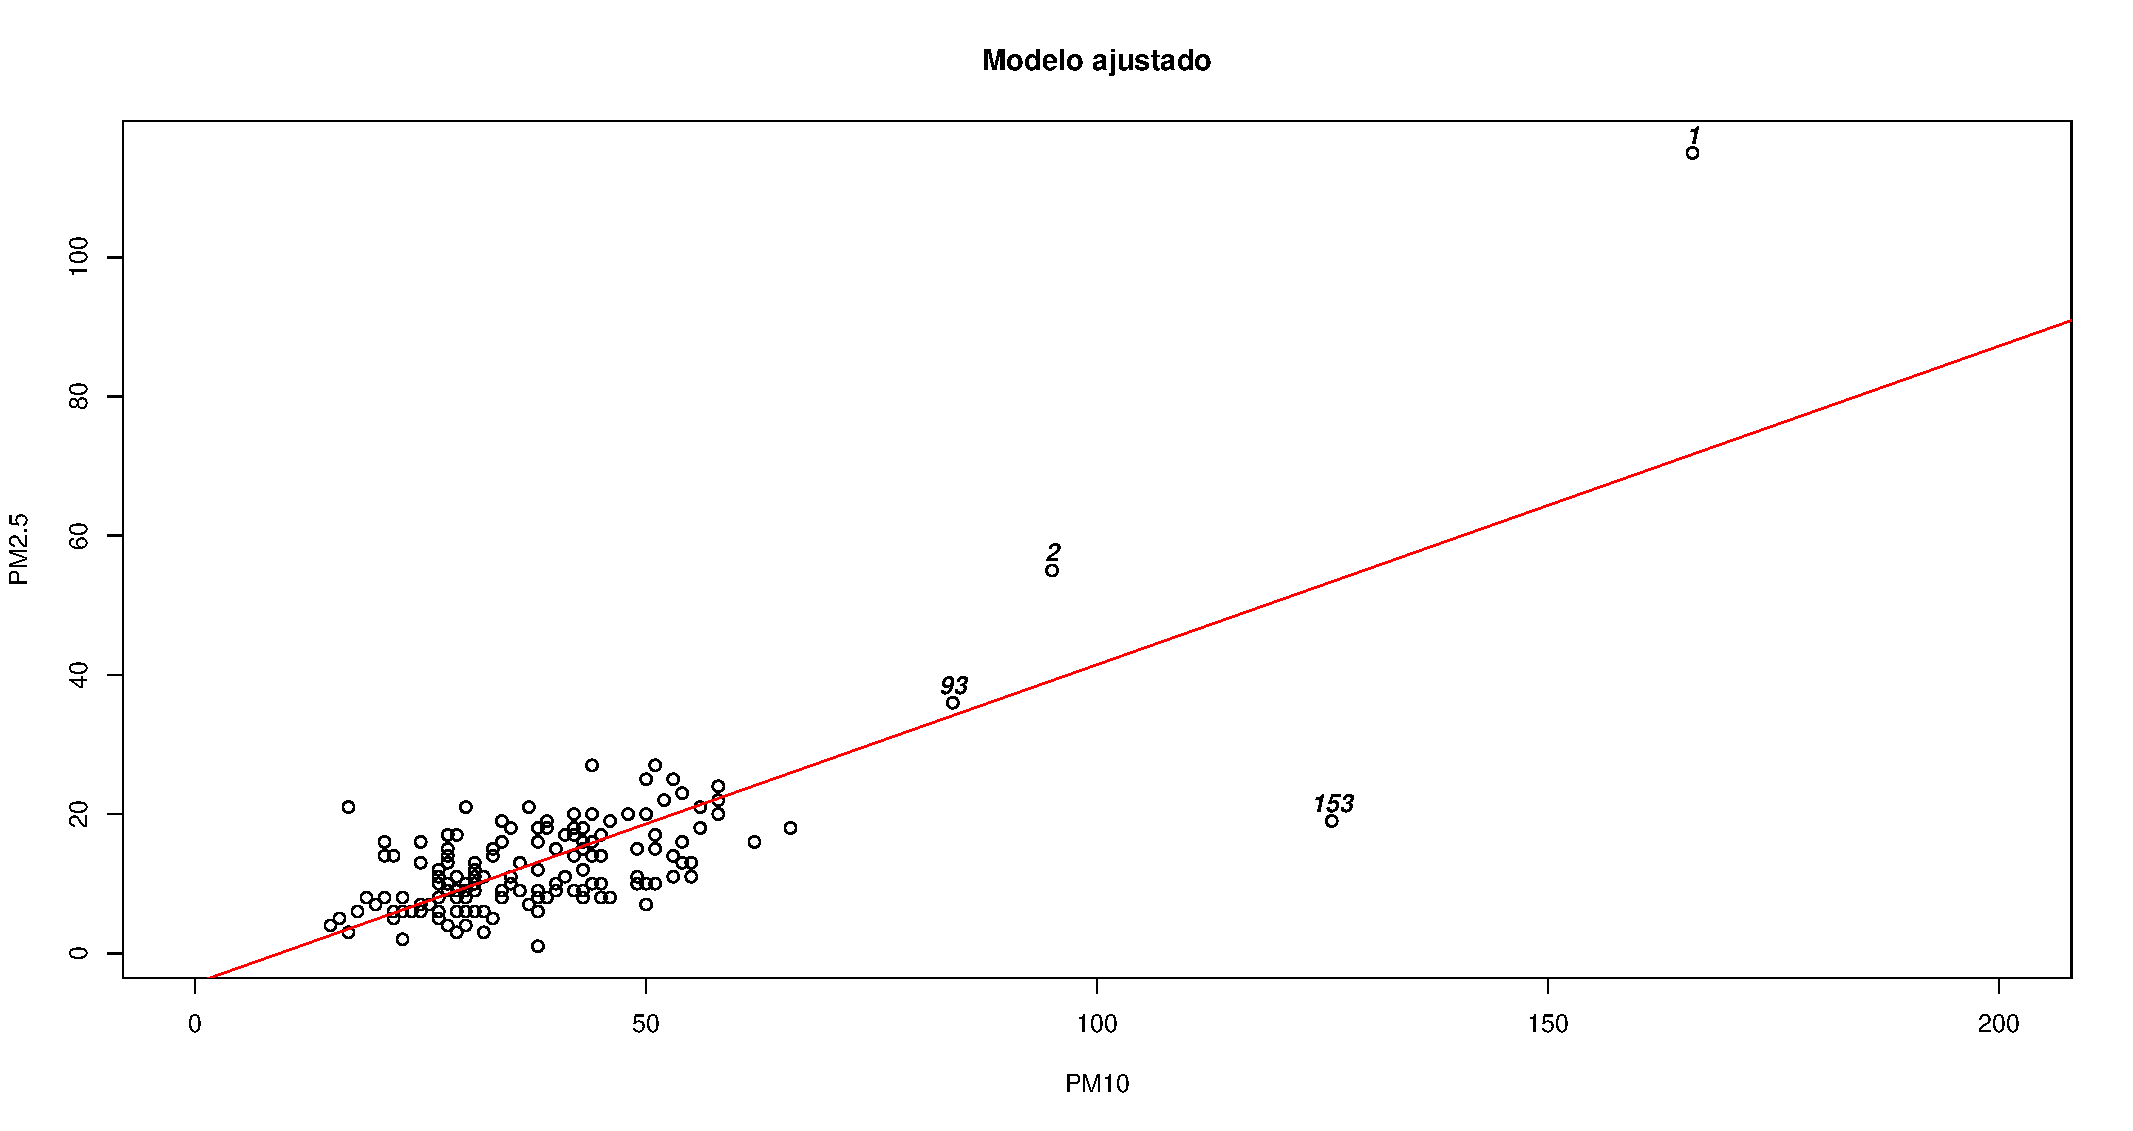
\includegraphics[scale=0.32]{imagenes/ma.pdf}
  \caption{Gráfico de dispersión con recta ajustada y valores candidatos a atipicos}\label{figura1}
\end{figure}
\end{itemize}
\end{frame}

\begin{frame}
\frametitle{Pruebas de diagnostico}
\begin{itemize}
\item[b)] \textbf{Gráfica de $\hat{d}$ vs $\hat{y}$:}
\begin{figure}[h]
  \centering
  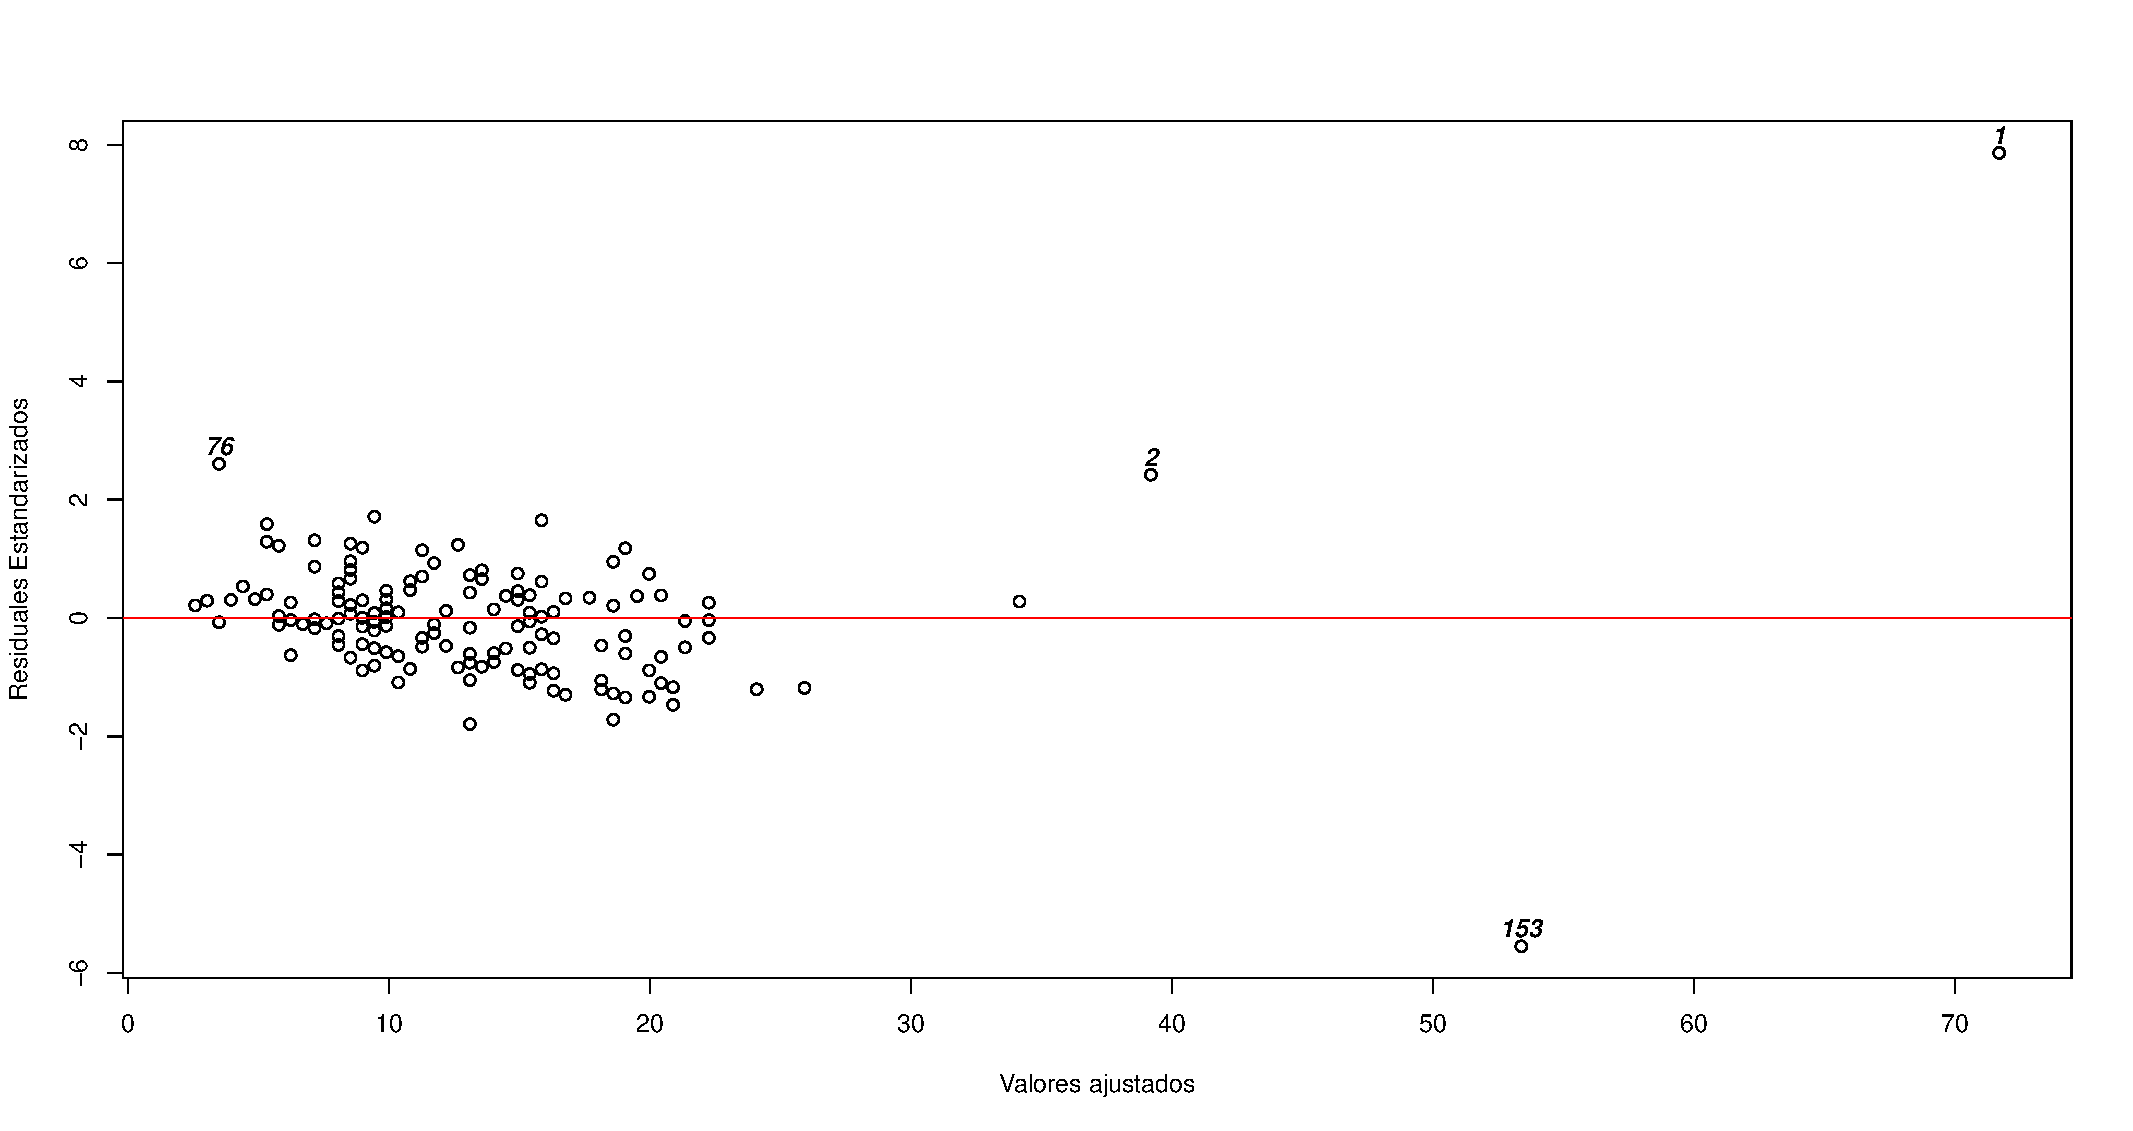
\includegraphics[scale=0.32]{imagenes/rv.pdf}
  \caption{Gráfico de residuales estandarizados vs los valores ajustados}\label{figura1}
\end{figure}
\end{itemize}
\end{frame}

\begin{frame}
\frametitle{Pruebas de diagnostico}
\begin{itemize}
\item[c)] \textbf{q-qplot de los residuales :}
\begin{figure}[h]
  \centering
  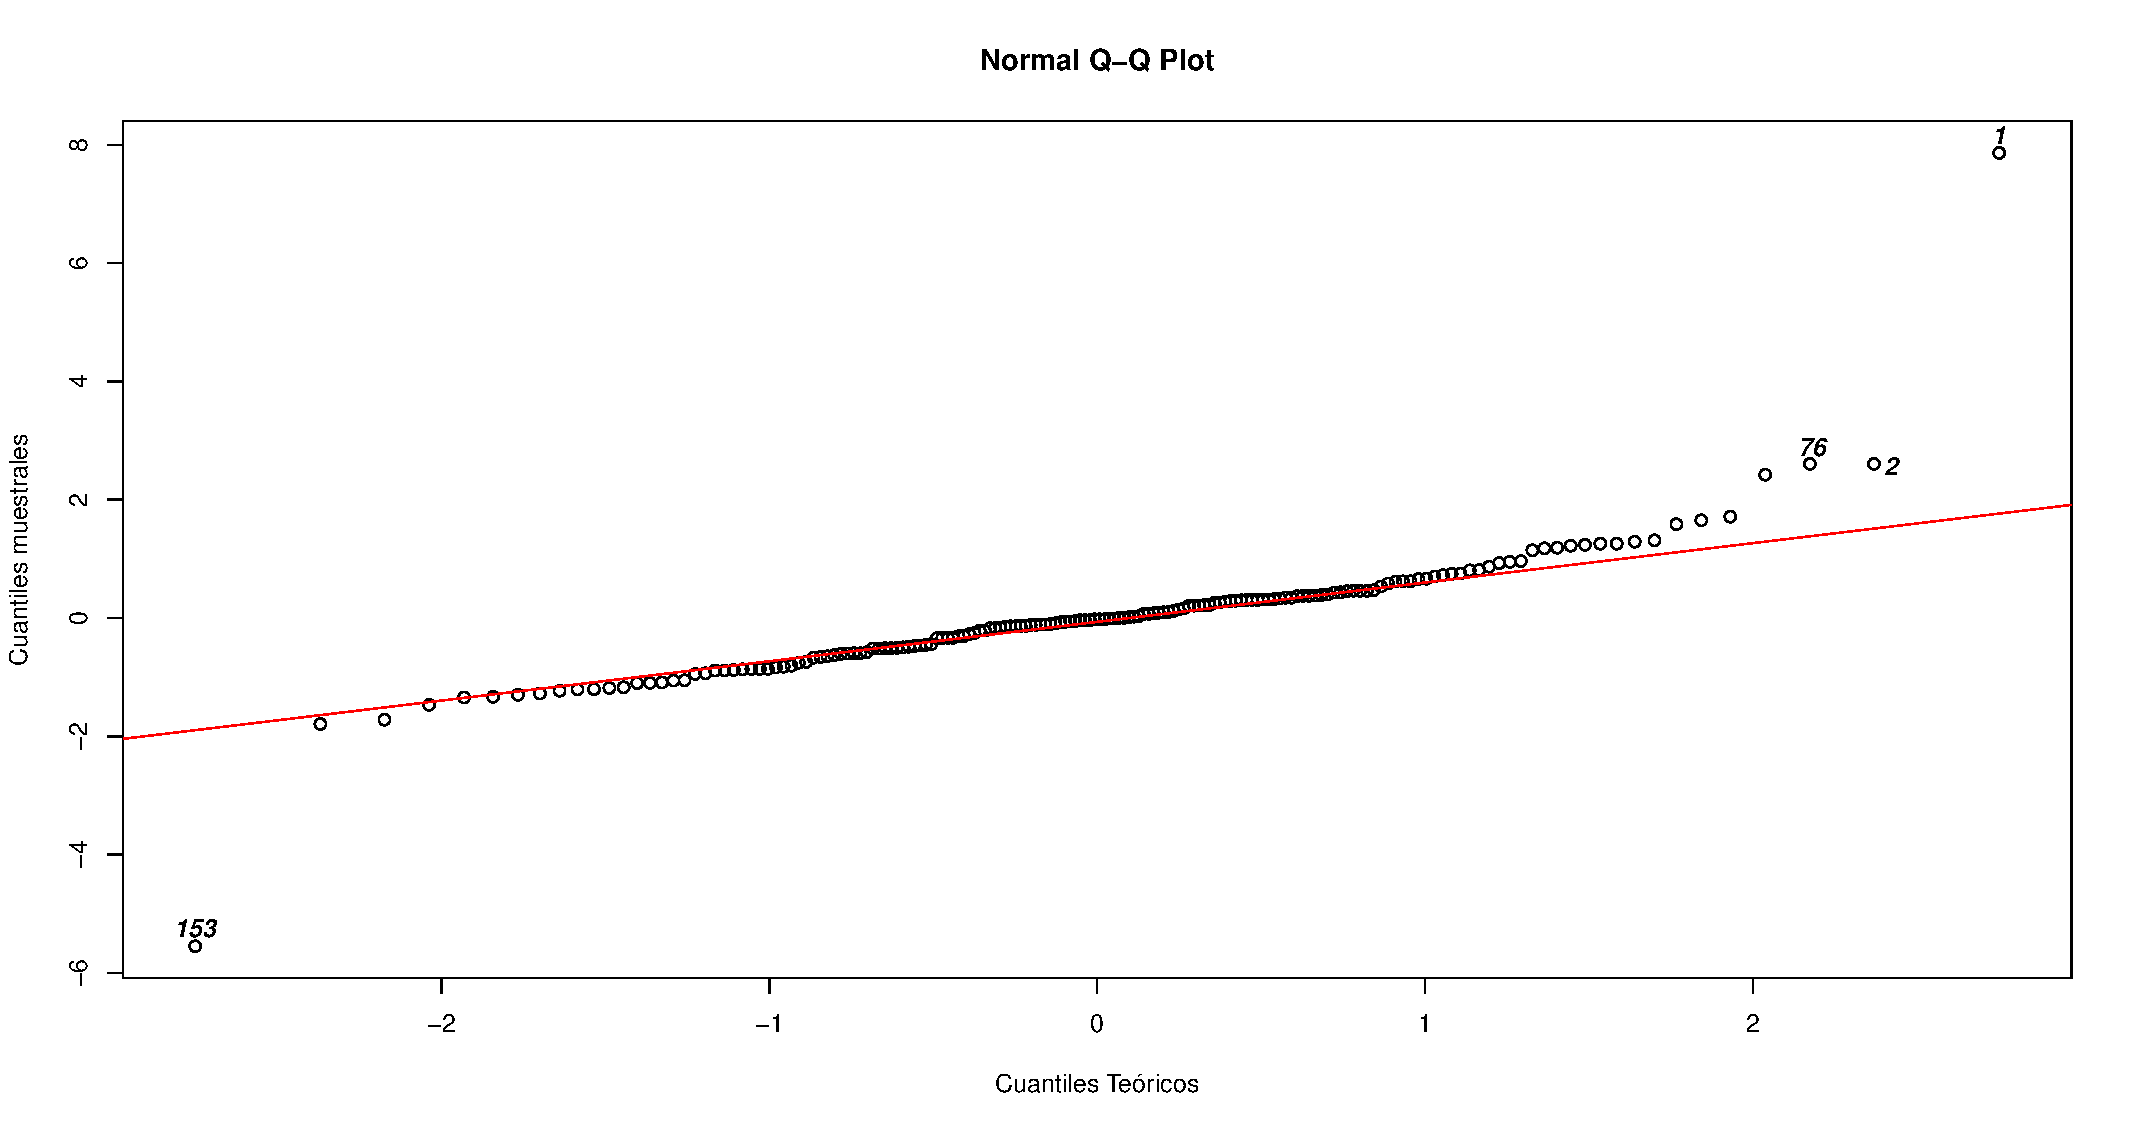
\includegraphics[scale=0.32]{imagenes/qq.pdf}
  \caption{q-qplot de los residuales}\label{figura1}
\end{figure}
\end{itemize}
\end{frame}

\begin{frame}
\frametitle{Pruebas de diagnostico}
\begin{itemize}
\item[d)] \textbf{Matriz HAT y residual Studentizado:} La matriz HAT definida como $H=x(x'x)^{-1}x^{T}$ y más específicamente el i-ésimo valor de su diagonal $h_{ii}=x'_{i}(X'X)^{-1}x_{i}$ y el residual Studentizado, definido como $\hat{r_{i}}=\frac{\hat{e_{i}}}{\sqrt{1-h_{ii}}\hat{\sigma}}$ sirven para ver si los puntos pueden ser influyentes o solo de balanceo, considerando los siguientes criterios:
\begin{itemize}
\item[-] Si $h_{ii}>\frac{2p}{n}=2\bar{h}=0.02381$ (como $\sum h_{ii}=p \rightarrow \bar{h}=\frac{p}{n}$) y el residual Studentizado es grande ($>3$), entonces la i-ésima observación puede considerarse influyente.
\item[-] Si solamente $h_{ii}>\frac{2p}{n}=0.02381$, entonces la i-ésima observación es solo de balanceo.
\end{itemize}
\end{itemize}
\end{frame}

\begin{frame}
\frametitle{Pruebas de diagnostico}
\begin{itemize}
\item[e)] \textbf{Distancia de Cook (D de Cook):} La distancia de Cook mide cómo cambia el vector de estimadores $\hat{\beta}$ cuando se elimina cada observación, por lo cuál es una medida útil para considerar como influyente una observación. La D de Cook se define como $D_{i}(M;C)=\frac{(\hat{\vec{\beta_{(i)}}}-\hat{\vec{\beta}})^T M(\hat{\vec{\beta_{(i)}}}-\hat{\vec{\beta}})}{C}$; i=1,...,n, donde $M=X^{T}X$ y $C=p\hat{\sigma^2}$. El criterio es:
\begin{itemize}
\item[-] Si $D_{i}\geq 1$, entonces la i-ésima observación puede considerarse como influyente.
\end{itemize}
\end{itemize}
\end{frame}

\begin{frame}
\frametitle{Pruebas de diagnostico}
\begin{itemize}
\item[f)] \textbf{DFFITS:} $DFFITS_{i}$ es la cantidad de desviaciones estándar que cambia el valor ajustado $\hat{y_{i}}$ si se elimina la observación i. Este criterio no define exactamente si el punto es influyente o de balanceo, solo sugiere que se debe examinar la observación. Se define como $DFFITS_{i}=\frac{\hat{y_{i}}-\hat{y_{(i)}}}{\sqrt{S^2_{(i)}}h_{ii}}$ El criterio es:
\begin{itemize}
\item[-] Si $|DFFITS_{i}|>2\sqrt{\frac{p}{n}}=0.2182$, sugiere que se debe investigar la influencia de la i-ésima observación.
\end{itemize}
\end{itemize}
\end{frame}

\begin{frame}
\frametitle{Pruebas de diagnostico}
\begin{itemize}
\item[g)] \textbf{DFBETAS:} Los $DFBETAS_{j,i}$ indica cuánto cambia el coeficiente de regresión $\hat{\beta_{j}}$ , en unidades de desviación estándar, si se omitiera la i-ésima observación. Esta se define como $DFBETAS_{ji}=\frac{\hat{\beta_{j}}-\hat{\beta_{j(i)}}}{\sqrt{S^{2}_{(i)}C_{jj}}}$ ; $C=(X^{T}X)^{-1}$. El criterio es:
\begin{itemize}
\item[-] Si $|DFBETAS_{ji}|>2/\sqrt{n}=0.1543$, entonces debe examinarse la i-ésima observación.
\end{itemize}
\end{itemize}
\end{frame}

\begin{frame}
\frametitle{Pruebas de diagnostico}
\begin{itemize}
\item[h)] \textbf{COVRATIO:} Esta medida sirve para expresar el papel de la i-ésima observación en la precisión de la estimación y se define como $\frac{|S^{2}_{(i)}(X^{T}_{i}X_{(i)})^{-1}|}{|S^{2}(X^{T}X)^{-1}|} $ ; i=1,2,...,n. El criterio es:
\begin{itemize}
\item[-] Si $COVRATIO_{i}>1$, entonces la i-ésima observación mejora la precisión de la estimación.
\item[-] Si $COVRATIO_{i}<1$, entonces la inclusión de la i-ésima observación disminuye la precisión de la estimación.
\item[-] Si $COVRATIO_{i}>1+3\frac{p}{n}=1.0357$  o si $COVRATIO_{i}<1-3\frac{p}{n}=0.9643$, entonces la i-ésima observación debería ser considerada influyente. 
\end{itemize}
\end{itemize}
\end{frame}

\begin{frame}
\frametitle{Resultados medidas de influencia}
\begin{center}
\resizebox{12.2cm}{!} {
\begin{tabular}{|cccccccc|}
\hline 
Observación & HAT & $\hat{r_{i}} $ &$D_{i}$ & $DFFITS_{i}$ & $DFBETAS_{(0),i}$ & $DFBETAS_{1,j}$ & $COVRATIO_{i}$ \\ 
\hline 
1 & 0.3384* & 9.8987499* & 15.8* & 7.07945* & -6.014452* & 7.02* & 0.602* \\ 
2 & 0.07179* & 2.4606893 & 0.227 & 0.684351* & -0.516887* & 0.655* & 1.015 \\  
76 & 0.01497 & 2.6539008 & 0.0516 & 0.327122* & 0.316146* & -0.254* & 0.945* \\  
79 & 0.01497 & 2.6539008 & 0.0516 & 0.327122* & 0.316146* & -0.254* & 0.945* \\ 
93 & 0.04881* & 0.2790688 & 0.00201 & 0.063217 & -0.044971 & 0.0592 & 1.063* \\ 
153 & 0.16301 & -6.1311115* & 3* & -2.705776* & 2.210180* & -2.66* & 0.802* \\ 
\hline 
\end{tabular} 
}
\end{center}
~\\Se puede observar que todas las observaciones de la tabla, se podrían considerar influyentes por uno u otro criterio.
\end{frame}

\begin{frame}
\frametitle{Modelo con intercepto 0}
~\\El modelo planteado para que pase por el origen es: 
$$PM_{2.5}=\beta_{1}PM_{10}$$
~\\El modelo ajustado asumiendo que el intercepto es igual a cero es: 
$$\hat{PM_{2.5}}=0.3638 PM_{10}$$
\end{frame}

\begin{frame}
\frametitle{Bondad del modelo}
~\\Para este modelo ajustado, tenemos los siguientes resultados que nos ayudaran a juzgar que tan bueno es:
\begin{center}
\begin{tabular}{|c|c|c|c|c|}
\hline 
 & Estimación & Desviación Estandár & Estadistico T & P valor \\ 
\hline 
$\beta_{1}$ & 0.3638 & 0.0129 & 28.2 & $<2e-16$ \\ 
\hline 
\end{tabular} 
\end{center}
\begin{center}
\begin{tabular}{|c|c|c|c|c|}
\hline 
$R^2$ & $R^2_{Ajustado}$ & $\hat{\sigma}$ & Estadistico F & Valor p \\ 
\hline 
0.8265 & 0.8254 & 6.978 & 795.4 & $<2.2e-16$ \\ 
\hline 
\end{tabular} 
\end{center}
\end{frame}

\begin{frame}
\frametitle{Comparación de modelos}
\begin{figure}[h]
  \centering
  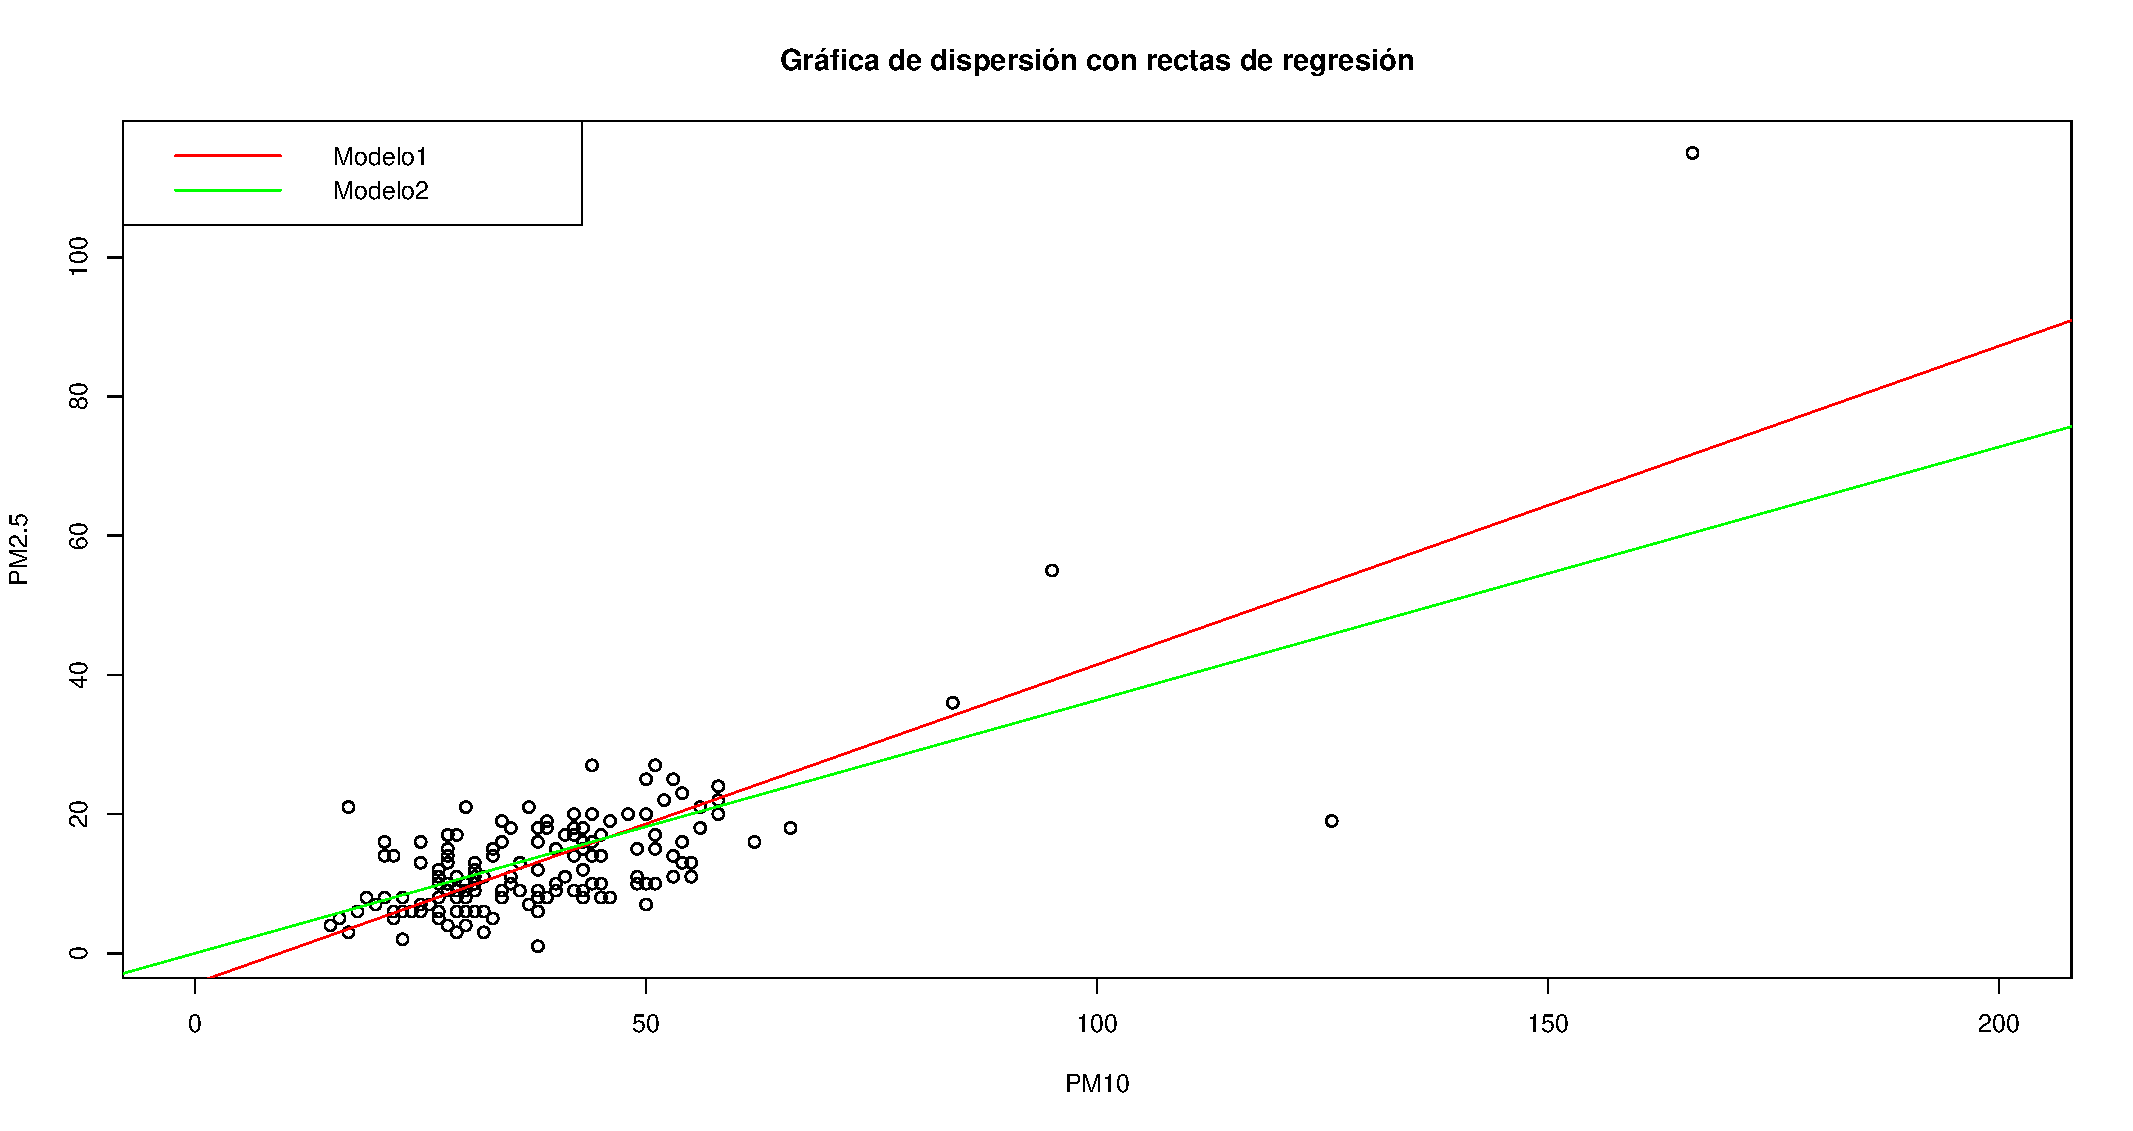
\includegraphics[scale=0.34]{imagenes/comp.pdf}
  \caption{Gráfica comparativa de rectas de regresión}\label{figura1}
\end{figure}
\end{frame}

\begin{frame}
\frametitle{Comparación de modelos}
~\\Para comparar los modelos tenemos la siguiente tabla comparativa:
\resizebox{12.2cm}{!} {
\begin{tabular}{|c|c|c|c|c|c|c|c|}
 \hline 
 Modelos & $R^{2}_{Ajustado}$ & $\hat{\sigma}$ & Estadistico F & Valor P & AIC & BIC & $SD(\beta_{1})$ \\ 
 \hline 
 Modelo 1 & 0.5729 & 6.7707 & 225 & $<2.2e-16$ & 1123.39 & 1132.762 & 0.03051  \\ 
 \hline 
 Modelo 2 & 0.8254 & 6.978 & 795.4 & $<2.2e-16$ & 1132.546 & 1138.794 & 0.0129\\ 
 \hline 
 \end{tabular}
 }  
\end{frame}

\begin{frame}
\frametitle{Comparación modelos}
~\\Seleccionamos como mejor modelo, al primero, en el cuál se ajusto con su intercepto, ya que los criterios de selección AIC y BIC dieron menores para este, además, la desviación del modelo a los datos es menor. Nos podría engañar en la selección el $R^2$ y el $R^2_{Ajustado}$, ya que estos aumentan casi en un $25\%$ lo cuál nos podría tentar a elegirlo como el mejor,este aumento ocurre ya que, al no haber intercepto, casi toda la variabilidad de Y ($PM_{2.5}$) es atribuible a X($PM_{10}$) eso explica el $R^2$ de $82\%$. Además, en el modelo sin intercepto $E(\hat{e})$ no es precisamente cero, en este caso esta cerca de -1, lo cuál es inadecuado.
\end{frame}

\begin{frame}
\frametitle{Pruebas de diagnostico modelo 2}
~\\Los resultados de las medidas de influencia y las pruebas de diagnostico para este modelo se resumen en la siguiente tabla:

\begin{center}
\resizebox{12.2cm}{!} {
\begin{tabular}{|ccccccc|}
\hline 
Observación & HAT & $\hat{r_{i}} $ &$D_{i}$ & $DFFITS_{i}$ & $DFBETAS_{1,j}$ & $COVRATIO_{i}$ \\ 
\hline 
1 & 0.094157* & 10.625441* & 7.03* & 3.43* &  3.43* & 0.661* \\ 
2 & 0.03084* & 3.048048* & 0.282 & 0.544* & 0.544* & 0.983 \\  
76 & 0.000987 & 2.146917  & 0.00446 & 0.0675 &  0.0675 & 0.980* \\  
79 & 0.000987 & 2.146917 & 0.00446 & 0.0675  & 0.0675 & 0.980* \\ 
93 & 0.024110* & 0.788304 & 0.0154 & 0.124  & 0.124 & 1.027* \\ 
153 & 0.054247* & -4.141674*  & 0.897 & -0.992*  & -0.992* & 0.964* \\ 
\hline 
\end{tabular} 
}
\end{center}
\end{frame}

\begin{frame}
\frametitle{Validación de supuestos, modelo con intercepto}
\begin{itemize}
\item[a)] Correcta especificación (Linealidad): Para evaluar la correcta especificación del modelo, simplemente nos basamos en las siguientes dos gráficas. 
\begin{figure}[h]
  \centering
  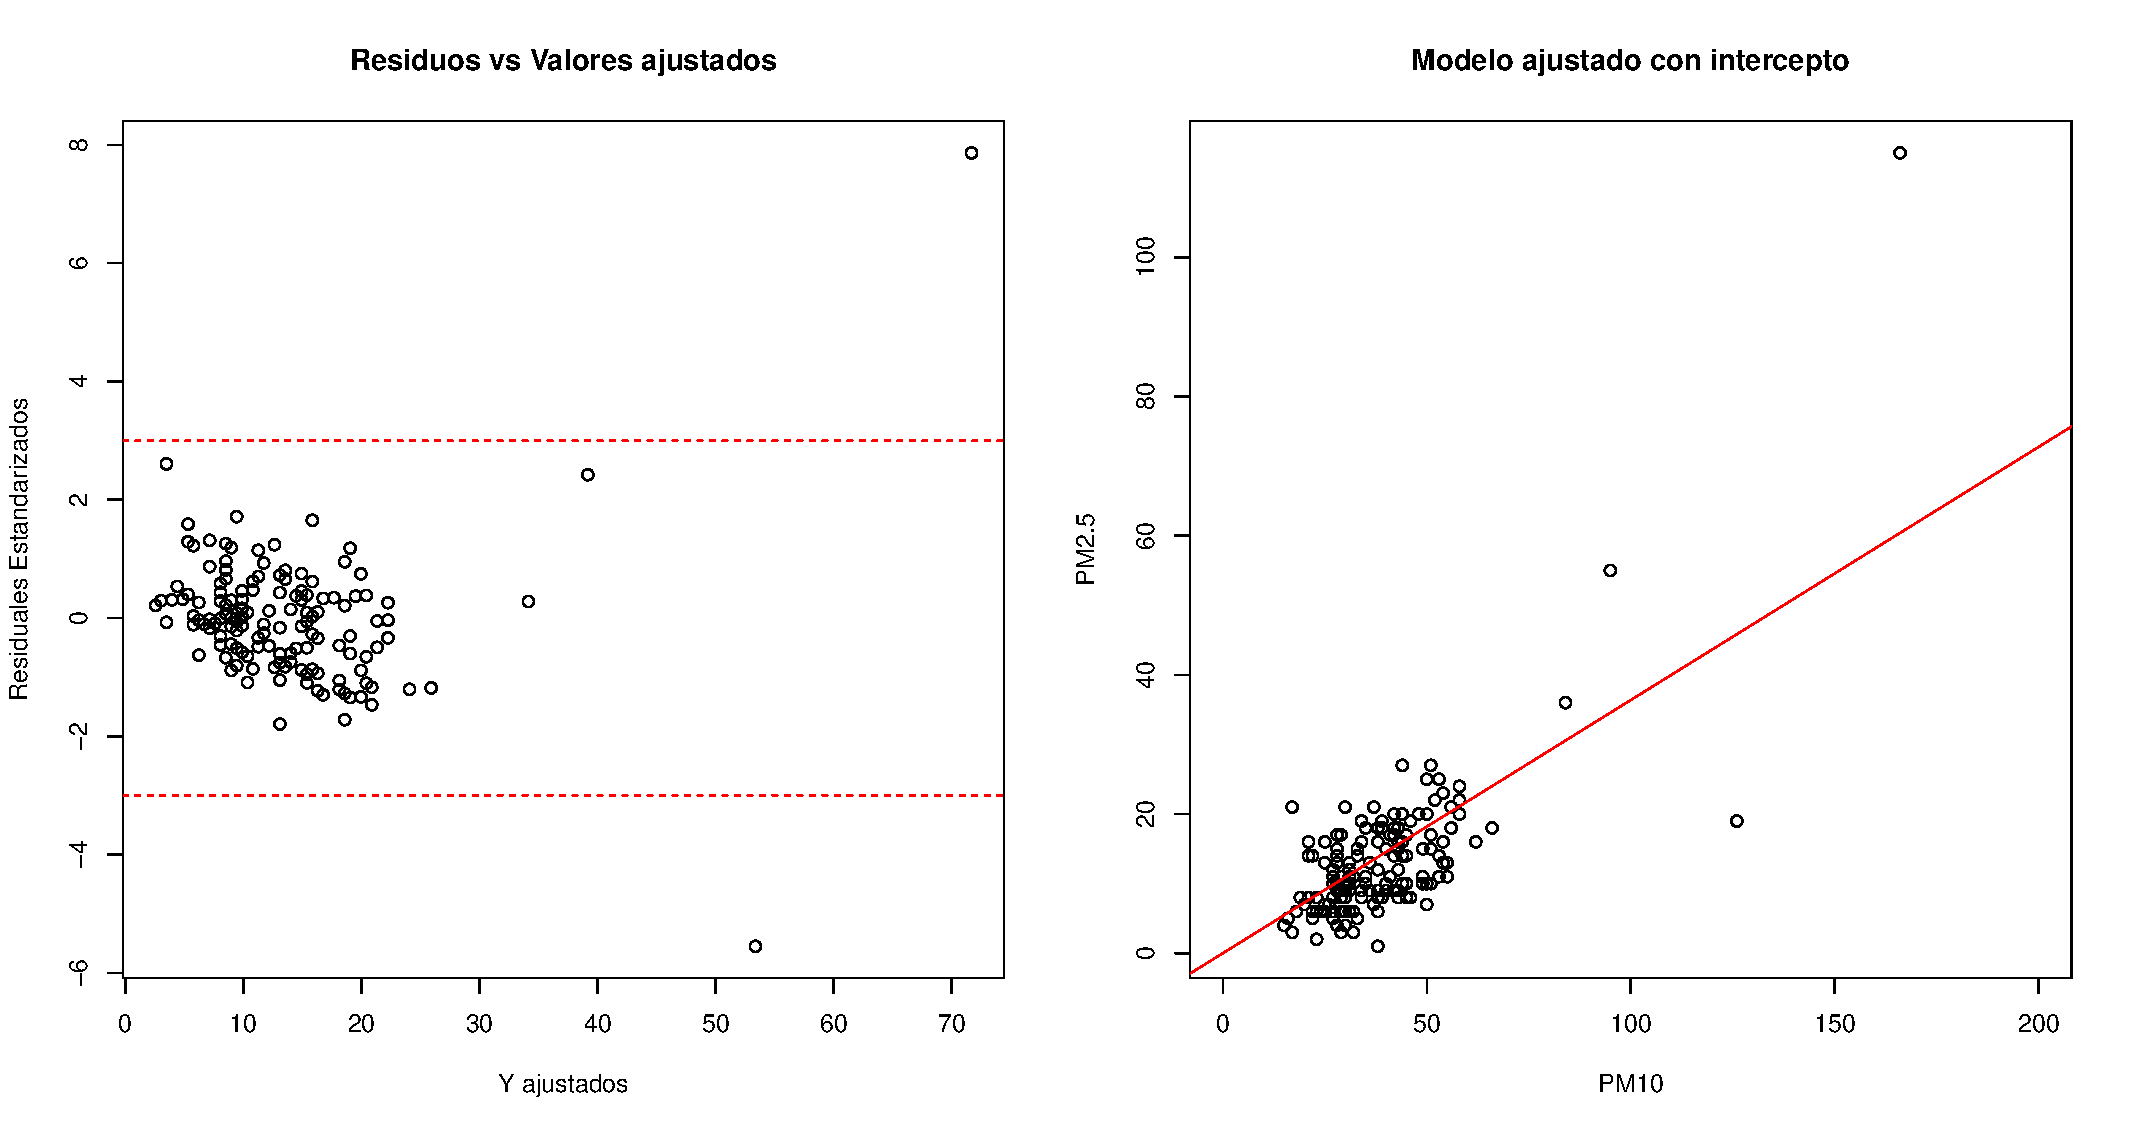
\includegraphics[scale=0.31]{imagenes/coresp.pdf}
  \caption{Gráficos para detectar incorrecta especificación }\label{figura1}
\end{figure}
\end{itemize}
\end{frame}

\begin{frame}
\frametitle{Validación de supuestos, modelo con intercepto}
\begin{itemize}
\item[b)] Normalidad de los errores: Para verificar este supuesto, se realizaron nuevamente dos gráficas, la primera, un histograma de los residuales para ver una posible forma de distribución de estos, y la segunda, el Q-Qplot, que muestra que tanto se asemeja la distribución de los residuales a la distribución normal. En ambas gráficas se evidencia que la distribución de los residuales no es normal, se puede ver en ambas que la cola derecha de la distribución de los residuales es mucho más pesada que en la distribución normal. Además aplicamos la prueba Shapiro-Wilk para confirmar nuestra creencia, esta prueba nos arrojo un estadístico de $W = 0.85121$ y un p valor= 8.796e-12, por tanto se rechaza $H_{0}$ y se concluye que la distribución de los residuales no es normal.
\end{itemize}
\end{frame}

\begin{frame}
\frametitle{Validación de supuestos, modelo con intercepto}
\begin{figure}[h]
  \centering
  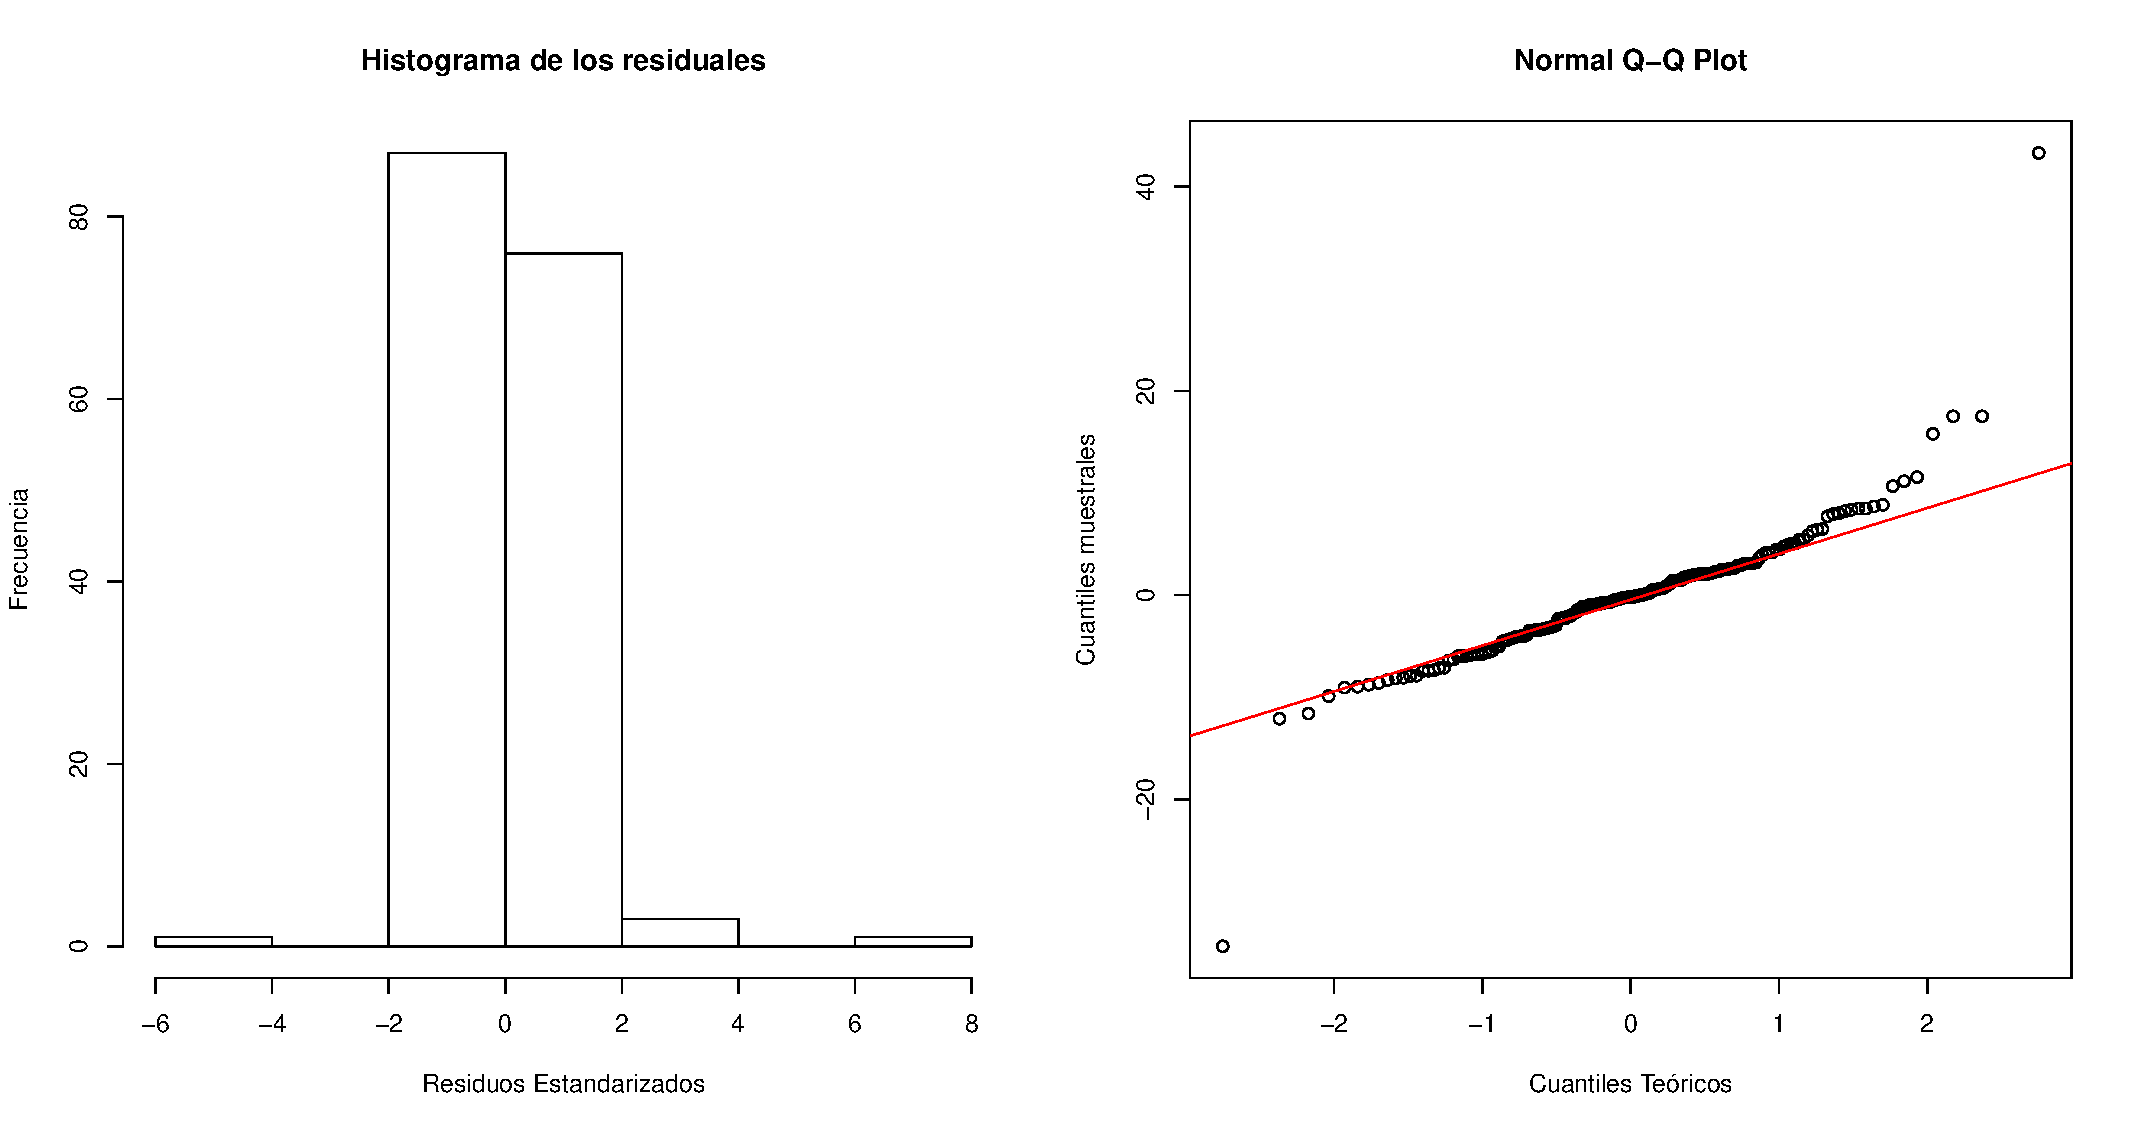
\includegraphics[scale=0.34]{imagenes/norm.pdf}
  \caption{Gráficos para evaluar la normalidad en los errores}\label{figura1}
\end{figure}
\end{frame}

\begin{frame}
\frametitle{Validación de supuestos, modelo con intercepto}
\begin{itemize}
\item[c)] Homocedasticidad: Para probar la homocedasticidad, se analiza la misma gráfica realizada en el literal a (los residuales vs los $\hat{y}$), donde no se ve claramente el incumplimiento de este supuesto, por lo cual se realizaron las pruebas Goldfeld-Quandt y Breusch-Pagan, se eligieron estas, ya que todas las otras pruebas más conocidas y utilizadas (Levene, Barlett, Cochran, etc) algunas requieren repeticiones en X y otros supuestos. La prueba Goldfeld-Quandt nos arrojo un estadístico de prueba $GQ = 0.6068$ y un p valor de 0.02487, y la prueba Breusch-Pagan nos arrojó un estadístico de prueba $BP = 83.079$ y un p valor asociado de aproximadamente 0 (< 2.2e-16). Por lo cuál en ambas pruebas se rechaza la hipótesis nula,y concluimos que los residuos del modelo no cumplen con el supuesto de homocedasticidad de varianza.
\end{itemize}
\end{frame}

\begin{frame}
\frametitle{Validación de supuestos, modelo con intercepto}
\begin{itemize}
\item[d)] Independencia en los errores: Sabemos que no se puede probar a ciencia cierta la independencia en los errores, sin embargo, para tener cierta idea sobre este supuesto, analizamos los residuales gráficamente (correlograma) y le aplicamos la prueba de Durbin Watson para darnos cuenta si estos tienen cierta correlación o dependencia. La prueba de Durbin-Watson nos arrojo un estadístico $DW = 1.1683$ y un p valor de 2.183e-08, entonces, para un nivel de significancia de 0.05, se rechaza $H_{0}$ y se concluye que la correlación entre los errores es diferente de cero.
\end{itemize}
\end{frame}

\begin{frame}
\frametitle{Validación de supuestos, modelo con intercepto}
\begin{figure}[h]
  \centering
  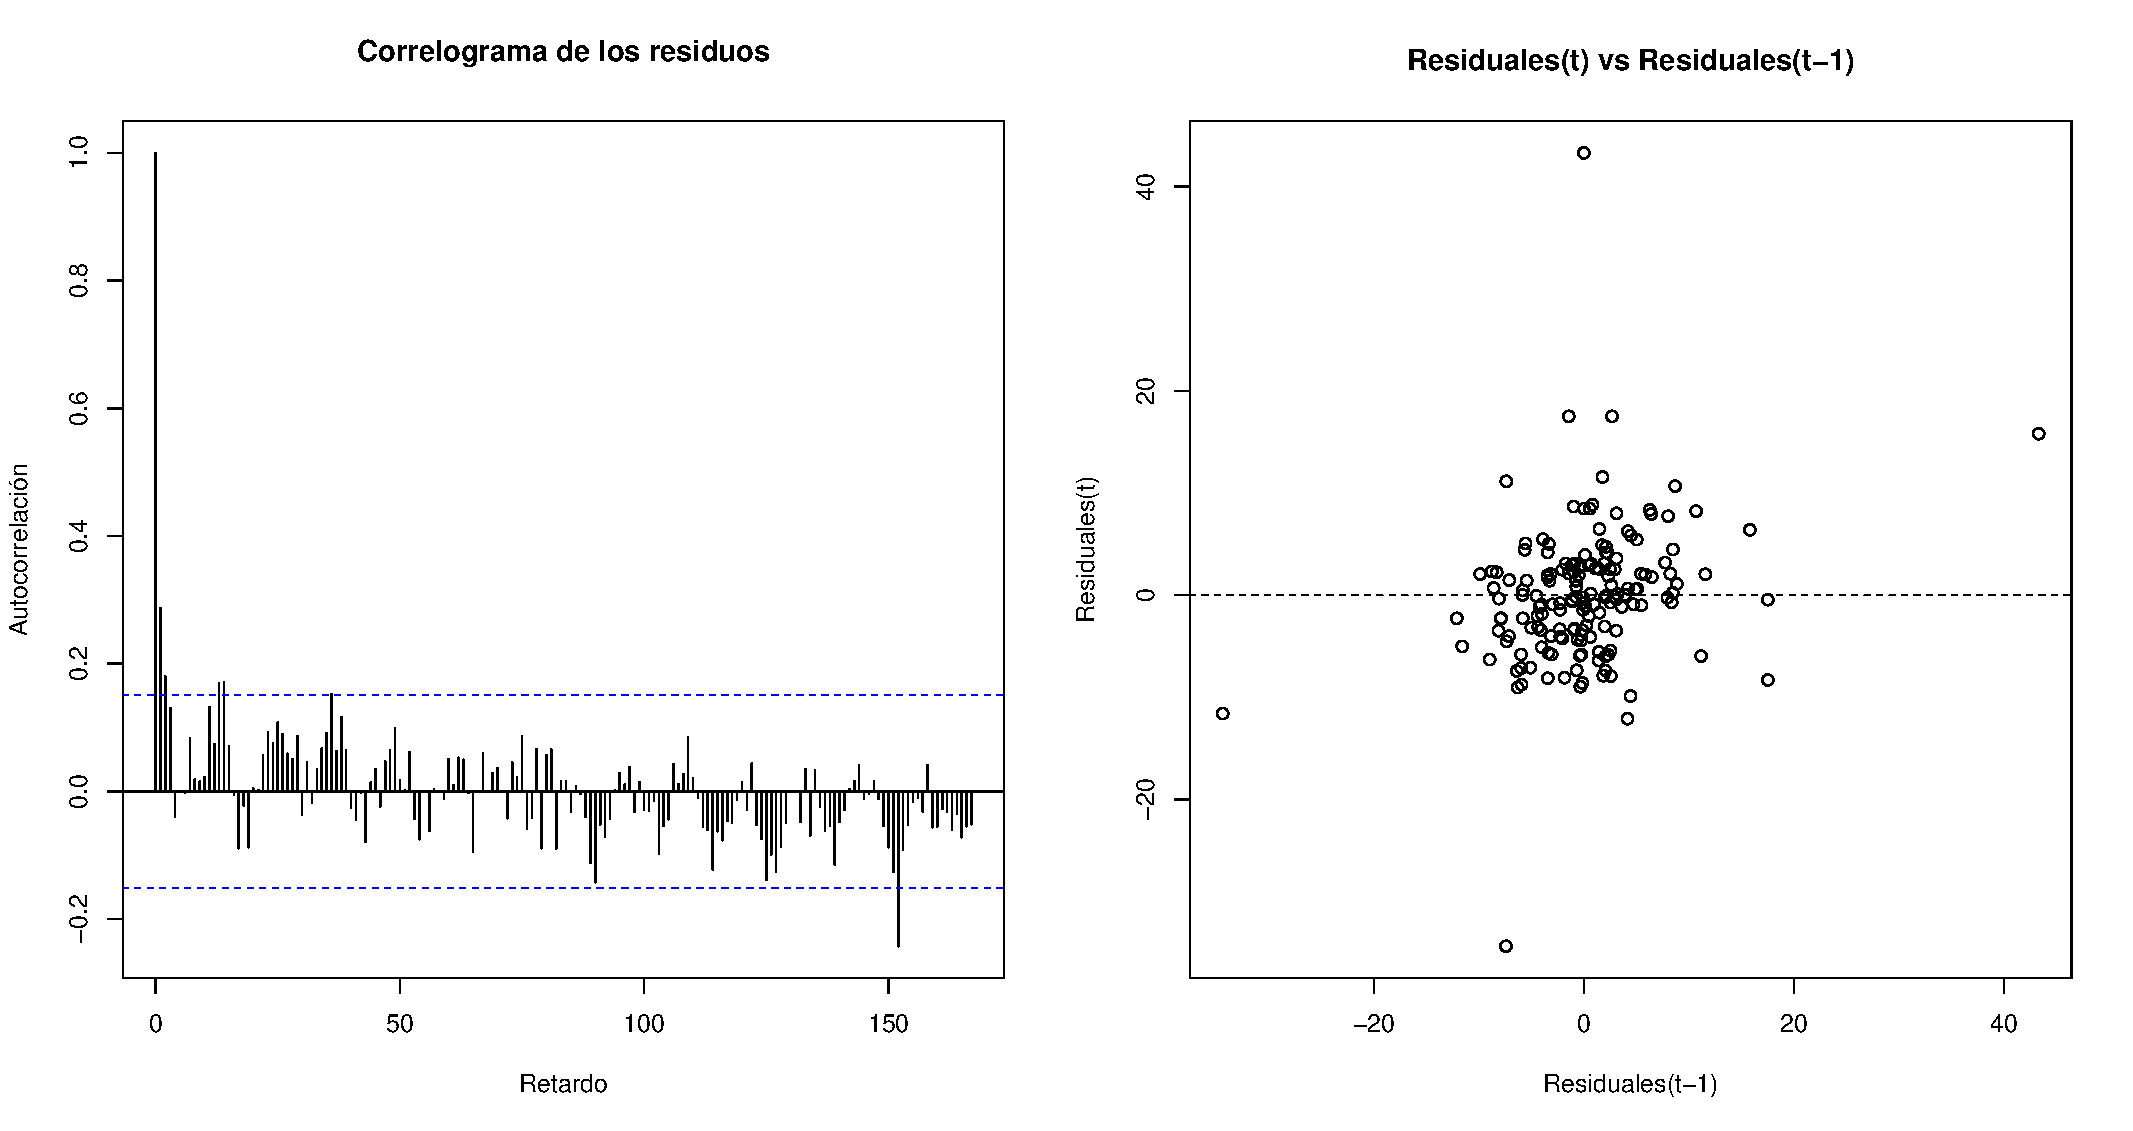
\includegraphics[scale=0.34]{imagenes/corr.pdf}
  \caption{Gráficos para evaluar la independencia en los errores}\label{figura1}
\end{figure}
\end{frame}

\begin{frame}
\frametitle{Regresión Robusta}
~\\Un proceso de regresión robusta es aquel que amortigua el efecto de las observaciones que serían muy influyentes si se usaran los mínimos cuadrados.
~\\Para aplicar regresión robusta existen varios métodos, entre lo más utilizados están:
\begin{itemize}
\item Método M (máxima verosimilitud): Le asigna una función de peso a los residuales, de forma que entre mayor sea el valor del residual menos peso le pone, por ende este método le da menos importancia a valores con residuales grandes.
\item Método LTS (Cuadrados menos recortados): Intenta minimizar la suma de residuos cuadrados.
\end{itemize}
\end{frame}

\begin{frame}
\frametitle{Regresión Robusta}
\begin{itemize}
\item Método S: Encuentra una línea (plano o hiperplano) que minimiza una estimación robusta de la escala (de la cual el método obtiene la S en su nombre) de los residuos.
\item Método MM: Intenta retener la solidez y la resistencia de la estimación S, mientras que gana la eficiencia de la estimación M. El método procede al encontrar una estimación S altamente robusta y resistente que minimiza una M-estimación de la escala de los residuos.
\end{itemize}
~\\Seleccionamos el método MM para la estimación de los coeficientes por ser el más robusto y el de mejor comportamiento, el modelo ajustado usando este método fue:
$$\hat{PM_{2.5}}=0.7196+0.3092 PM_{10}$$

\end{frame}

\begin{frame}
\frametitle{Regresión Robusta}
\begin{figure}[h]
  \centering
  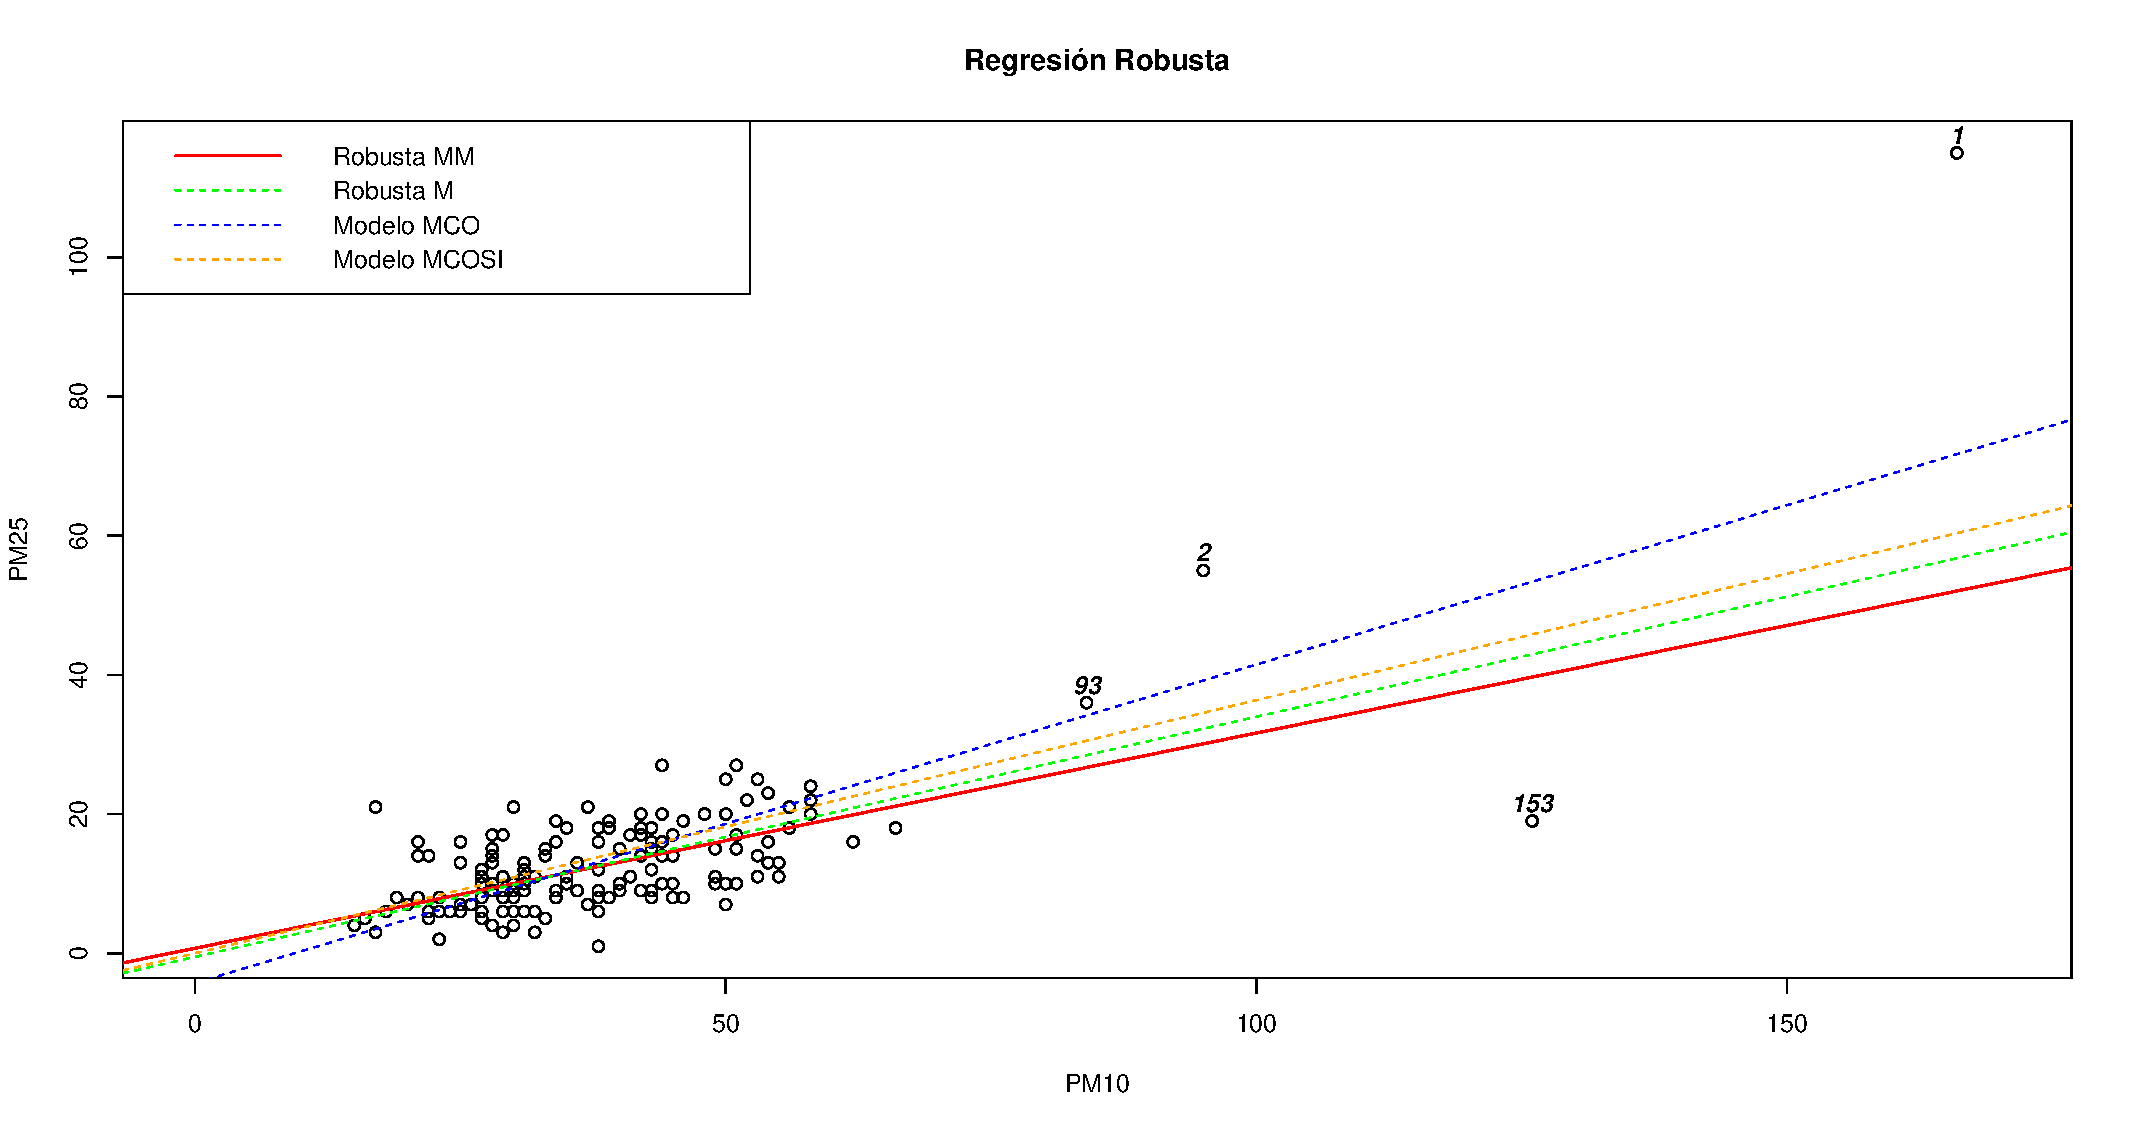
\includegraphics[scale=0.34]{imagenes/robusta.pdf}
  \caption{Gráficos para evaluar la independencia en los errores}\label{figura1}
\end{figure}
\end{frame}

\begin{frame}
\frametitle{Bondad del modelo}
~\\Para este modelo ajustado, tenemos los siguientes resultados que nos ayudaran a juzgar que tan bueno es:
\begin{center}
~\\\begin{tabular}{|c|c|c|c|c|}
\hline 
 & Estimación & Desviación Estandár & Estadistico T & P valor \\ 
\hline 
$\beta_{0}$ & 0.7196 & 0.9259 & 0.7771 & 0.4382 \\ 
\hline 
$\beta_{1}$ & 0.3092 & 0.0222 & 13.9372 & 0 \\ 
\hline 
\end{tabular} 
\end{center}
\begin{center}
\begin{tabular}{|c|c|c|}
\hline 
 $\hat{\sigma}$ & AIC & BIC \\ 
\hline 
 4.824 & 1147.121 & 1156.493 \\ 
\hline 
\end{tabular} 
\end{center}
\end{frame}

\begin{frame}
\frametitle{Comparación de modelos}
~\\Para comparar los modelos tenemos la siguiente tabla comparativa:
\resizebox{12.2cm}{!} {
\begin{tabular}{|c|c|c|c|c|c|c|c|}
 \hline 
 Modelos & $R^{2}_{Ajustado}$ & $\hat{\sigma}$ & Estadistico F & Valor P & AIC & BIC & $SD(\beta_{1})$ \\ 
 \hline 
 Modelo 1 & 0.5729 & 6.7707 & 225 & $<2.2e-16$ & 1123.39 & 1132.762 & 0.03051  \\ 
 \hline 
 Modelo 2 & 0.8254 & 6.978 & 795.4 & $<2.2e-16$ & 1132.546 & 1138.794 & 0.0129\\ 
 \hline 
 Modelo Robusto &    & 4.824 &  &  & 1147.121 & 1156.493 & 0.0222 \\
 \hline 
 \end{tabular}
 }  
~\\Podemos concluir que el mejor modelo es el último (Regresión Robusta), ya que, el criterio de comparación entre un modelo MCO y un modelo Robusto es la varianza del modelo, el cambio de los coeficientes de regresión y las desviaciones de esos coeficientes.
\end{frame}

\begin{frame}
\frametitle{Conclusión}
~\\Podemos ver que la desviación del modelo disminuyó de 6.7707 a 4.824,los coeficientes estimados cambiaron considerablemente y las desviaciones de las estimaciones también disminuyeron considerablemente. En este caso, no se toma muy en cuenta el AIC y el BIC, ya que estos criterios no se pueden usar para comparar modelos obtenidos por métodos diferentes (MCO y Regresión Robusta). Además, es muy razonable elegir el modelo ajustado por regresión robusta, ya que los supuestos del modelo 1 no se cumplen, por lo cuál las estimaciones por MCO y en general la teoría de los Mínimos Cuadrados Ordinarios es inadecuada y no se debe usar al no cumplirse sus supuestos. 
\end{frame}
\end{document}